\section*{Method}

Our design imposes additional structure on top of existing machine learning
approaches, enforcing properties on the reconstructed values. For functions \[ f(p, t)\to\mathbb{R}^n, t\in[0,1] \] which is modelled through
a learned approach, we decompose it into a function: \[ f(p)\to\mathbb{R}^{n\times O}, B_O(f(p), t)\to\mathbb{R}^n
\] Where
$O$ is the order of the Bezier spline, $f(p)$ is the learned control points, and $B_O(f(p), \cdot)$ is the evaluation
of the $O$th order Bezier spline with control points defined by $f(p)$.

\subsection*{Architecture}

Specifically for dynamic NeRF, $f(p)$ is defined as
$\text{MLP}(x,y,z)\to\mathbb{R}^{3\times O}$. We ray march from a camera with known position and
view direction through the scene, and at every point we compute the set of control points for a Bezier curve. We then evaluate the Bezier curve at a given time, and deform the ray by the result, producing some $\Delta_0(x)$. The number of spline points for the Bezier curve is hyperparameter, but we are able
to accurately reconstruct movement with as low as 4 spline points, but experiment with 16 spline points. In order to evaluate the Bezier curve in a numerically stable way, we use De Casteljau's
algorithm. In a future extension, we plan on extending it to handle rational Bezier splines, which would allow for even greater control of movement.

De Casteljau's algorithm evaluated at time $t$ is characterized by the recurrence relation:
\[ \beta_i^{(0)} = \beta_i, \]
\[ \beta_i^{j} = (1-t)\beta_i^{(j-1)} + t\beta_{i-1}^{(j-1)}, \]
which can be thought of as linearly interpolating between adjacent control points until there is only a single point remaining. This takes $O(n^2)$ operations to evaluate, where $n$ is the number of control points.

We are also interested in constructing a reasonable canonical NeRF, and arbitrarily select $t = 0$ to be canonical. Thus, we are interested in Bezier Curves where $B_O(0) = \overrightarrow{0}$. This can be achieved in two different ways, either by assigning $p_0 = \overrightarrow{0}$, and only computing the other control points: $f(p) = p_{1\cdots O-1}$. Then, we can use the Bezier spline with the control points as the concatenation of $\overrightarrow{0}$ with the other control points: $[\overrightarrow{0}, p_{1\cdots O-1}]$. Alternatively, we can compute $p_{0\cdots O-1}$ and use the Bezier spline with control points but subtract the first predicted point from all of them: $[p_{0\cdots O-1}]-p_0$, and the final change in position is $\Delta_0(x) = B_O(f(p)-f(p)_0,t)+p_0$. While both formulations are in theory equivalent and explicitly concatenating $\overrightarrow{0}$ leads to fewer degrees of freedom, we find the second approach leads to better convergence near $t=0$, so we use that.

Following NR-NeRF, we also learn how rigid each ray is, which in theory should allow more efficient learning of which regions are space are fixed. This rigidity $\in[\epsilon, 1]$)is computed as a function of position:
\[ \text{Rigidity} =\sigma_{\epsilon^\uparrow}(\text{MLP}(x)), \]
\[ \sigma_{\epsilon^\uparrow}(v) = \sigma(v)(1-\epsilon) + \epsilon, \]
where $\sigma$ is defined as the sigmoid function $\frac{1}{1+e^{-x}}$. Rigidity rescales the
difficulty of learning movement, making it more easy to represent and classify static scene
objects. The final change in position is defined as $\Delta(x) = \text{Rigidity}\times
\Delta_0(x)$.

In order to reconstruct RGB values, we also diverge from the original NeRF, and only allow for
positional dependent colors:
\[ \text{RGB} = \sigma_{\epsilon-\text{wide}}(\text{MLP}(x)) \]
\[ \sigma_{\epsilon-\text{wide}}(v) = \sigma(v)(1+2\epsilon) - \epsilon \]
using the activation function as described in MIP-NeRF~\cite{barron2021mipnerf} in order to prevent vanishing gradients on colors. Because of the low number of
samples for a moving object at a given view, it is more difficult to learn specular
reflection, thus it leads to better convergence to model the diffuse color of an object. This is in line with NR-NeRF and D-NeRF, which also model the diffuse component.

A diagram of the ray-bending component can be seen in Fig.~\ref{fig:arch_diagram}.

\begin{figure}
    \centering
    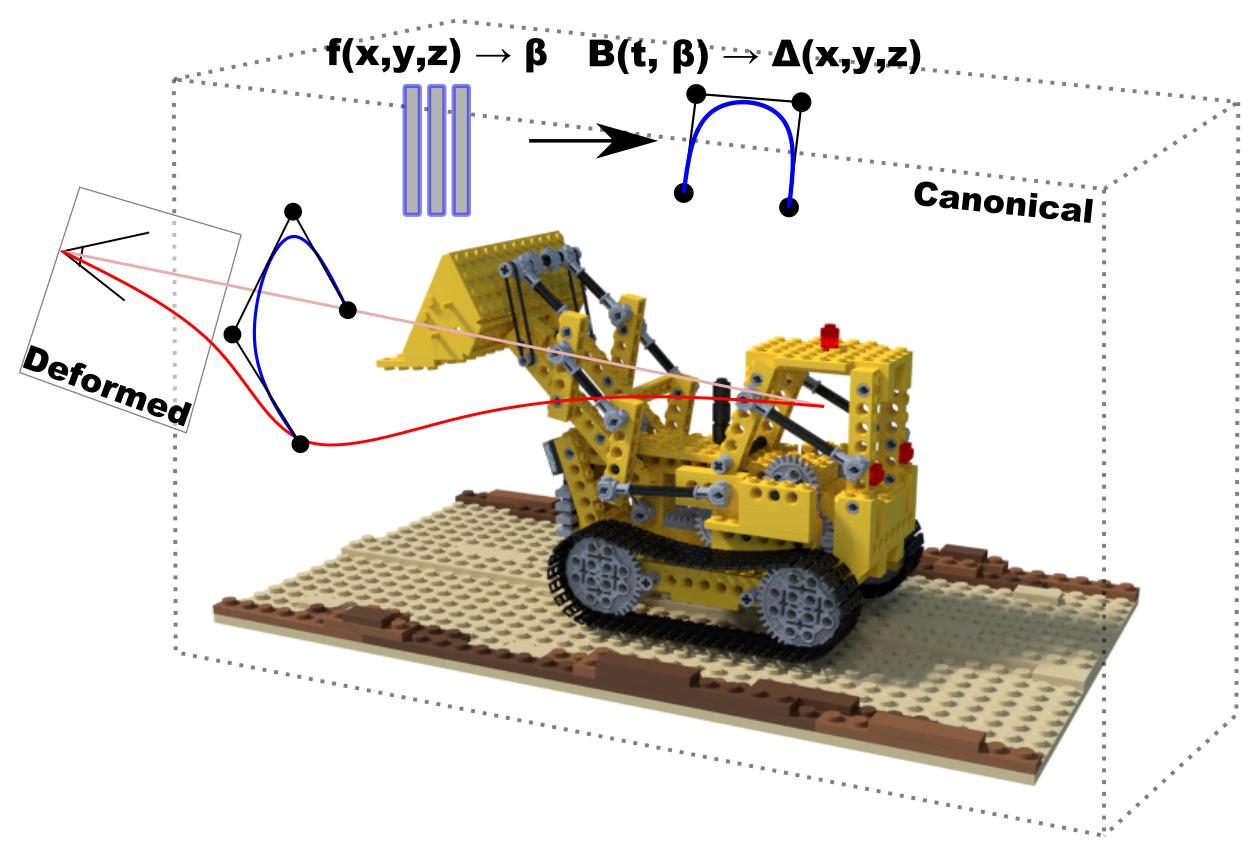
\includegraphics[width=0.5\textwidth]{spline_nerf_diagram.png}
    \caption{
        \textbf{Spline-based Dynamic NeRF}. Instead of using an MLP to directly predict ray-bending at a given time, we predict a set of Bezier spline control points. Then, we use the Bezier function to interpolate position based on time.
    }
    \label{fig:arch_diagram}
\end{figure}

\subsection*{Training}

For training, we sample random crops of random frames, computing the loss defined previously and back-propagating through the whole network. We use autograd to optimize control points and the canonical NeRF jointly, but note that there are also classical approaches to solving spline points which may lead to faster optimization in the future. We use the Adam optimizer~\cite{Kingma2015AdamAM} with cosine simulated annealing~\cite{loshchilov2017sgdr} to go from $\num{2e-4}$ to $\num{5e-5}$ over the course of a day.

For some scenes, we are able to have higher learning rates, but for much darker scenes it's necessary to lower the learning rate to converge.

\iffalse
\subsection*{Loss}

While training, we introduce another loss term, as the $\ell_2$ loss may have
difficulty when there is a large pixel-wise gap in movement between the learned and predicted
component. $\ell_2$ may also miss large structural differences between two images if they are close in color, so we add a loss function which is high for incorrect structure of an image.

The new loss term is \[
    L_\text{FFT} = \text{MSE}(\text{FFT}(I_\text{GT}), \text{FFT}(I_\text{predicted}))
\],
where the FFT is the 2D fast Fourier transform of an image.
MSE is the mean squared error in the complex domain as the FFT has both a real and imaginary component, and is defined as \[ \text{MSE}(a\in\mathbb{C}^k,b\in\mathbb{C}^k) \]
\[ = \frac{1}{k}\Sigma_{i=0}^k|a_i-b_i| \]
\[ |z\in\mathbb{C}| = (\Re(z)+\Im(z))(\Re(z)-\Im(z)) \]
We introduce this term as a cheap replacement to structural similarity (SSIM), since the
FFT captures information about the structure of the whole image, which is useful in a dynamic setting due to the disjointedness of where a predicted object may be as opposed to its final position\footnote{In a published iteration, we would likely perform an ablation of this loss function.}.

Our final loss formulation is:
\[ \ell_2(I_\text{predicted}, I_\text{GT}) + L_\text{FFT}(I_\text{predicted}, I_\text{GT}) \]
without any additional regularization terms.

Our formulation is simpler compared to NR-NeRF since there is no need to regularize
temporal consistency, making the optimization process simpler. Our training process also does not require adding in additional frames over time for short sequences, so we randomly sample from all available frames. This is contrast to D-NeRF, which requires adding frames in during training since it has to enforce that at $t=0$ the predicted movement is 0.

\subsection*{Long Duration $C^0$ Continuity}

While the above structure is sufficient to model short-term $C^0$ continuity, it runs into
numerical instability and higher cost the longer the sequence is, due to the $O(n^2)$
evaluation cost of De Casteljau's algorithm. To deal with this, we design an additional architecture which
composes the previous architecture for many small $C^0$ curves. Concatenating many small splines permits for reconstruction of infinitely long sequences with guaranteed $C^0$-continuity with only a few additional models.

The architecture is based off of poly-splines, or a composition of many small Bezier splines.
For a known-length sequence, we divide it into $K$ segments, and assume that $K$ evenly divides the total number of frames. We can then treat $t$ as is
in the range $[0, K]$, and $t$ can be decomposed into a segment number and fractional component:
\[ k\in\mathbb{Z}_K=\lfloor t\rfloor, t'\in[0,1)=t-k \]
Then we define an embedding $\text{Emb} = \mathbb{R}^{Z\times(K+1)}$, where $Z$ is a latent
dimension size. We then create an "anchor" network:
\[
    \textit{anchor}(x\in\mathbb{R}^3,z\in\mathbb{R}^Z) = \text{MLP}(x,z)\to(\mathbb{R}^3,\mathbb{R}^{Z'})
\]
We call it an "anchor" network because it computes
endpoints which anchors each of the curves, and also computes a representative latent vector. Between these two
endpoints, we are interested in computing $O-2$ intermediate spline points. We define the
control point estimation network as
\[
\textit{control}(x\in\mathbb{R}^3, z_1, z_2\in\mathbb{R}^{Z'}) = \text{MLP}(x,z_1,z_2)\to\mathbb{R}^{O\times\mathbb{R}^3}
\]
Where $z_1,z_2$ are the
representative latent vectors from the anchor network, and it outputs $O-2$ spline points in
$R^3$. We can also include a per-segment rigidity value, similar to above, but lose
some guarantees of continuity by doing so.

In order to evaluate the network at a given time $t$ and other inputs $x$, we first compute $k, t'$. Then, we compute
the anchor points at
\[ p_0,z_1=\textit{anchor}(x,\text{Emb}[k]) \]
\[ p_\text{end},z_2=\textit{anchor}(x,\text{Emb}[k+1]) \]
and the intermediate control points as \[ p_{1\cdots O-2} = \text{control}(x,z_1,z_2) \]
The final set of control points we use
is the concatenation of the anchors with the intermediate points:
$[p_0, p_{1\cdots O-2}, p_\text{end}]$. Using this set of control points, we evaluate the Bezier
curve spline at $t'$ using De Casteljau's algorithm:
\[ \text{De Casteljau}([p_0, p_{1\cdots O-2}, p_\text{end}], t) = \Delta(x) \]
Because we are evaluating adjacent embeddings ($k, k+1$) for each anchor, we are guaranteed that the endpoints between each spline segment are identical. Information is also carried over between segments through the anchor's
representative latent vector, allowing the network to maintain velocity between curves if necessary.

This architecture enforces a guarantee of consistency, regardless of how long a reconstructed signal is. It also naturally allows movement at one time to be distinct from another,
as while the endpoints of the spline are fixed, movement defined by the intermediate control points is allowed to be fully independent of other
segments. While we construct this architecture for long dynamic sequence reconstruction, we argue that it works more generally for generating $C^0$-continuous functions in any domain.

One obvious question is why a more complex architecture is necessary as compared to predicting all spline points and using only some of them. In the case of extremely long sequences, the number of spline points may increase linearly with the length of the function, and for dynamic NeRF we would have memory cost of $O(H\times W\times D\times t)$ which is prohibitively expensive. With the proposed architecture, we are able to sample sparsely, maintaining a constant memory usage with respect to time.

We do yet not demonstrate the effectiveness of the architecture, due to time constraints, and the author's incompetence\footnote{If this were to be published, I would demonstrate this architecture, but cannot due to time constraints.}.
\fi

\subsection{Voxel Spline-NeRF}

In addition to a model that uses an MLP to predict the control points, we demonstrate that using control points is also effective for voxelized NeRF, which leads to much faster reconstruction times. Our formulation is identical